\chapter{Конструкторский раздел}


\section{Углы Эйлера}
\hspace{0.6cm} Углы Эйлера определяют три поворота системы, которые позволяют привести любое положение системы к текущему. Обозначим начальную систему координат как (x, y, z) , конечную как (X,Y,Z). Пересечение координатных плоскостей xy и XY называется линией узлов N.
\begin{itemize}
	\item Угол a между осью x и линией узлов — угол прецессии.
	\item Угол b между осями z и Z — угол нутации.
	\item Угол y между линией узлов и осью  X— угол собственного вращения.
\end{itemize}

\hspace{0.6cm} Повороты системы на эти углы называются прецессия, нутация и поворот на собственный угол (вращение). Такие повороты некоммутативны и конечное положение системы зависит от порядка, в котором совершаются повороты. В случае углов Эйлера производится серия из трёх поворотов:
\begin{enumerate}
	\item На угол a вокруг оси z. При этом ось x переходит в N.
	\item На угол b вокруг оси N. При этом ось z переходит в Z.
	\item На угол y вокруг оси Z. При этом ось N переходит в X.
\end{enumerate}

\hspace{0.6cm} Иногда такую последовательность называют 3,1,3 (или Z,X,Z), но такое обозначение может приводить к двусмыслице.
\hspace{0.6cm} Для вычисления этих углов используются векторы. Генеральная идея если у нас есть 3 точки P1(X1, Y1, Z1),  P2(X2, Y2, Z2),  P3(X3, Y3, Z3) состоит в том что бы найти 2 вектора (Вектор $\vec{P_{1}P_{2}}$ и вектор $\vec{P_{2}P_{3}}$) что бы найти угол между ними. Чтобы найти эти 2 вектора мы воспользуемся формулой

\begin{equation} 
\displaystyle \vec{AB} = (X_2 – X_1, Y_2 – Y_1, Z_2 – Z_1)\\
\vec{BC} = (X_3 – X_2, Y_3 – Y_2, Z_3 – Z_2) 
\end{equation}

\hspace{0.6cm} Так как существует формула:

\begin{equation} 
\displaystyle  \vec{AB} \cdot \vec{BC} = |\vec{AB}| \cdot |\vec{BC}| * \cos(\theta),
\end{equation}

\hspace{0.6cm} где $\theta$ – угол между этими векторами, то из этой формулы мы получаем этот угол помощу arccos. Длину вектора находим по формуле:

\begin{equation} 
\displaystyle  |\vec{AB}| = \sqrt{(X_{AB}^2 + Y_{AB}^2 + Z_{AB}^2)}.
\end{equation}

\hspace{0.6cm} Конечная формула получается:

\begin{equation} 
\displaystyle  \theta = \arccos(\frac{\vec{AB} * \vec{BC}}{|\vec{AB}| * |\vec{BC}|}).
\end{equation}

\hspace{0.6cm} Если мы хотим найти угол по оси X или оси Y, то мы просто не включаем эти координаты у уравнение, т.е. если хотим например найти по оси X то вектор $\vec{P_{1}P_{2}}$ можем вычислить вот так:
\begin{equation} 
\displaystyle  \vec{P_{1}P_{2}} = (0, Y_2 - Y_1, Z_2 - Z_1).
\end{equation} 
	

\section{Структура проверок положения точек}
\hspace{0.6cm} Входные данные в программу представляют собой 42 точки в трехмерном пространстве. Из 42 точек, 21 определяет одну кисть.

\hspace{0.6cm} Проверка кисти на правильность осуществляется с помощью группы проверок отдельных пальцев, а также точек расположенных непосредственно на ладони. Для реализации проверок лучше использовать язык программирования Prolog, поскольку это мощный инструмент именно для работы с логическими конструкциями.

\hspace{0.6cm} Для удобства представления входных данных их можно разделить на структуры. 

\begin{figure}[ht!]
	\centering
	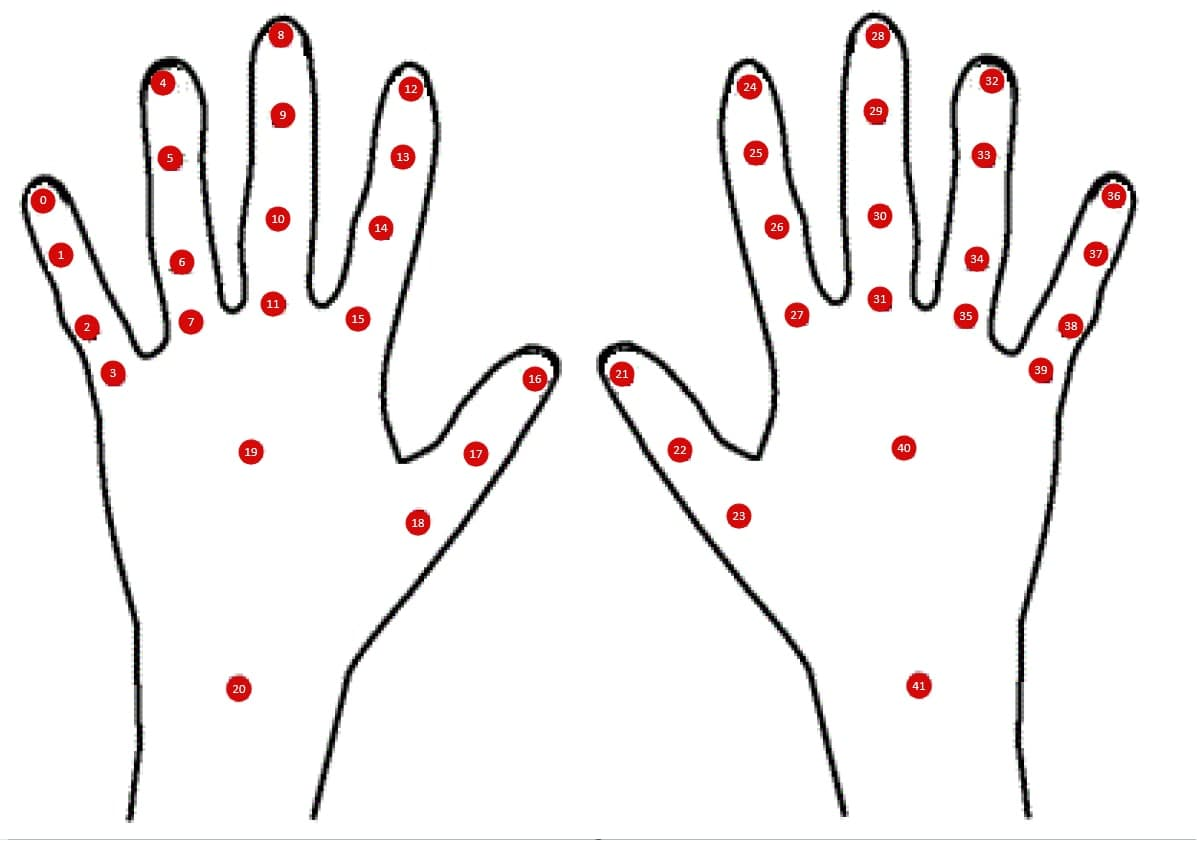
\includegraphics[scale=0.5]{Kist.jpg}
	\caption{Нумерация точек на кисти}
	\label{fig:hands}
\end{figure}

\hspace{0.6cm} Возьмем точки 0, 1, 2, 3. Вместе они составляют мизинец на руке. В соответствии с этим можно создать структуру мизинца. Схожим образом можно объединить оставшиеся точки в безымянный, средний, указательный и большой пальцы. Останутся только точки 19, 20 на левой руке и 40, 41 на правой. Эти точки являются ключевыми для своих кистей соотвественно.

\hspace{0.6cm} Далее полученные структуры пальцев мы можем объединить в структуру руки. Каждая рука будет состоять из пальцев и оставшимся двум точкам соответственно для левой и правой кисти.

\hspace{0.6cm} Данные преобразования необходимо провести для упрощения понимания структуры кода при его чтении, а также облегчения работы при написании процедур проверок.

\hspace{0.6cm} Сами проверки в своей основе опираются на проверку углов между определенными точками в пальце.  

\hspace{0.6cm} Мы создали структуры проверок для всех пальцев в Прологе, где проверяли является ли угол между тремя точками меньше или больше предполагаемого, и если да то это положение недопустимо. При этом мы находили углы по оси X и по оси Y так как:
\begin{itemize}
	\item Сгибание - Это когда три точки создают угол по оси X от 0 до -180;
	\item Разгибание -Это когда три точки создают угол по оси X от 0 до 180;
	\item Отведение - Это когда три точки создают угол по оси Y от 0 до -180;
	\item Приведение - Это когда три точки создают угол по оси Y от 0 до 180;
\end{itemize}

\hspace{0.6cm}Эта проверка вызывается 2 раза для обе руки.

\hspace{0.6cm} Как можно увидеть из таблицы \ref{tab:amplitude_finger}, у нас различаются углы для большого пальца, 4 остальных пальцев и самой ладони. Поэтому мы сделали 3 различные структуры проверок.

\hspace{0.6cm} Если какие то проверки не проходят допустимость, то мы записываем эти точки в текстовой файл что бы питон потом мог отобразить не допустимые кости руки.

\hspace{0.6cm} Структуру мы разбили на несколько частей: Три точки -> Палец -> Рука

\hspace{0.6cm} Структуру трёх точек мы представляем как Point(X, Y, Z)

\hspace{0.6cm} Для пальца мы сделали 5 структуру для каждого из них:
	
\begin{lstlisting}[caption=Листинг структур пальцев, label=struct:finger]
	finger(little, P0, P1, P2, P3),
	finger(ring, P4, P5, P6, P7),
	finger(middle, P8, P9, P10, P11),
	finger(index, P12, P13, P14, P15),
	finger(thumb, P16, P17, P18)
\end{lstlisting}
\hspace{0.6cm} где P – это номер точки на руке.

\hspace{0.6cm} Для руки мы сделали структуру:
\begin{lstlisting}[caption=Листинг структуры руки, label=struct:hand]
Hand
(
	finger(little, P0, P1, P2, P3),
	finger(ring, P4, P5, P6, P7),
	finger(middle, P8, P9, P10, P11),
	finger(index, P12, P13, P14, P15),
	finger(thumb, P16, P17, P18),
	P19, P20
)
\end{lstlisting}

\hspace{0.6cm} где $P_{i}$ - точка на руке, $i$ – это номер точки на руке.

\hspace{0.6cm} Так как углы допустимости одинаковы для пальцев 2, 3, 4, 5, то для них мы сделали одинаковую проверку.

\section{Визуализация руки}

\hspace{0.6cm} Визуализация руки написана на python, с использованием библиотек TkInter и OpenGL. Для визуализации руки нам нужно приложение, которое может загружать точки из текстового файла, а так же редактировать уже имееющиеся точки с помощью мышки ради изменения их положения.

\hspace{0.6cm} TkInter – Библиотека для Питона, которая позволяет создавать интерфейс.

\hspace{0.6cm} OpenGL – API для разработки для рендеринга 3д и 2д графики. Оно позволяет нам вместе с Tkinter визуализировать кисть руки, и показать инвалидные ребра этой кисти. С помощью OpenGL мы избавились от большого количества формул и алгоритмов, которые бы нам потребовались, если бы мы сами писали свой движок.

\hspace{0.6cm} Точки будем брать из текстового файла, которых должно быть 42. После проверки допустимости мы будем рендерить руки на экран. Если при проверке будут найдены точки, которые не прошли проверку, надо их запомнить, а при рендеринге их ребра будем окрашивать красный цвет. Точки будем изображать черными квадратами.

\begin{figure}[ht!]
	\centering
	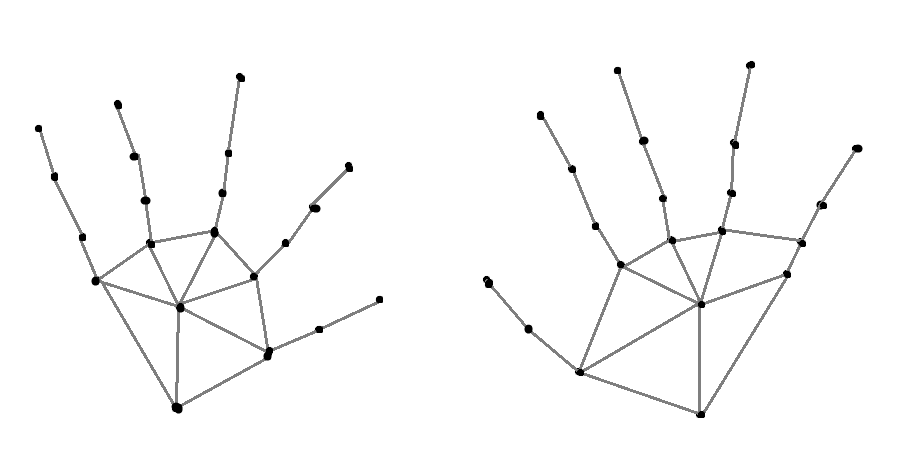
\includegraphics[scale=0.65]{schematic.png}
	\caption{Схематическое изображение желаемого результата рендеринга}
	\label{fig:example4}
\end{figure}
	

